  Im Kapitel Projektadministration wird eine Detailanalyse der Aufgabenstellung
  durchgeführt. Daraus abgeleitet wird die Planung definiert. Zusätzlich gibt es
  Informationen über die einzelnen Arbeitsschritte und den Erreichungsgrad der
  gestellten Aufgaben.
  
  \section{Detailanalyse der Aufgabenstelltung}

  In der Detailanalyse der Aufgabenstellung werden die definierten Aufgaben der
  Aufgabenstellung untersucht und deren Resultate ausgearbeitet. Aufgrund dieser
  Erkenntnisse wird eine Grobplanung festgelegt. Damit die Nachvollziehbarkeit
  garantiert ist, werden die Termine, Meilensteine und Arbeitsschritte
  aufgelistet.
  
  \begin{description}
    \item[Aufgabe - A1\label{itm:Aufgabe-01}]
    \begin{itshape}Analyse bestehender Java Swing Applikationen der Zürcher
    Kantonalbank.\end{itshape}
    \item[Im Detail\label{itm:Detail-01}]
    Es sollen die gängigen Mechanismen von Java Swing Applikationen der Zürcher
    Kantonalbank untersucht werden. Das soll aus der Sicht des Anwenders
    passieren. In drei bestehenden Java Swing Applikationen soll die Existenz
    bekannter GUI Paradigmen untersucht werden.
    \item[Resultat - R1\label{itm:Resultat-01}]
    Es soll eine Liste der erkannten Paradigmen vorliegen.
  \end{description}
  
  \begin{description}
    \item[Aufgabe - A2\label{itm:Aufgabe-02}]
    \begin{itshape}Erkennen und Kategorisieren der verwendeten
    Swingkomponenten.\end{itshape}
    \item[Im Detail\label{itm:Detail-02}]
    Die drei ausgewählten Java Swing Applikationen werden genauer betrachtet.
    Es wird das Augenmerk auf die Verwendung von Swingkomponenten gelegt. Diese
    sollen über die drei Applikationen hinweg konsolidiert und kategorisiert
    werden.
    \item[Resultat - R2\label{itm:Resultat-02}]
    Es soll eine Liste der verwendeten Swingkomponenten vorliegen.
  \end{description}
  
  \begin{description}
    \item[Aufgabe - A3\label{itm:Aufgabe-03}]
    \begin{itshape}Evaluation von Java Web Frameworks, welche sich am Markt
    etabliert haben.\end{itshape}
    \item[Im Detail\label{itm:Detail-03}]
    Es soll ein Evaluationsverfahren gewählt werden, bei dem eine möglichst
    objektive Entscheidung gefällt werden kann. Welche Java Web Frameworks in
    die Evaluation miteinbezogen werden, soll über Recherchen im Internet und in
    Büchern geschehen. Es sollen fünf Java Web Frameworks gewählt werden, welche
    anhand der Recherchen für valable Optionen in Frage kommen. Über die
    Definition von Soll- und KO-Kriterien sollen die Rahmenbedigungen für das
    Evaluationsverfahren geschaffen werden. Anhand der ausgearbeiteten
    Evalautionsmethode soll gezeigt werden, wie geeignet die Java Web Frameworks
    wirklich sind.
    \item[Resultat - R3\label{itm:Resultat-03}]
    Es soll eine Rangliste der fünf Frameworks, in der Anordnung entsprechend
    ihrer Eignung, vorliegen.
  \end{description}
  
  \begin{description}
    \item[Aufgabe - A4\label{itm:Aufgabe-04}]
    \begin{itshape}Prüfen, ob eine Integration der evaluierten Java Web
    Frameworks, welche für eine Umsetzung geeignet sind, in der bestehenden IT
    Infrastruktur der Zürcher Kantonalbank möglich ist.\end{itshape}
    \item[Im Detail\label{itm:Detail-04}]
    Gemäss den Vorgaben der IT Infrastruktur der Zürcher Kantonalbank, soll ein
    mögliche Einsatz der evaluierten Java Web Frameworks geprüft werden. Die
    meisten Java Web Frameworks haben in ihrer Dokumentation die Anforderungen
    definiert, welche für einen möglichen Betrieb nötig sind. Aufgrund dieser
    Anforderungen, und der bestehenden IT Infrastruktur soll ein Vergleich
    gemacht werden.
    \item[Resultat - R4\label{itm:Resultat-04}]
    Es sollen die Java Web Frameworks aufgelistet werden, welche für einen
    Einsatz in der IT Infrastruktur der Zürcher Kantonalbank in Frage kommen.
  \end{description}
  
  \begin{description}
    \item[Aufgabe - A5\label{itm:Aufgabe-05}]
    \begin{itshape}Prüfen, ob eine Implementierung der erkannten
    Swingkomponenten in den evaluierten Java Web Frameworks möglich
    ist.\end{itshape}
    \item[Im Detail\label{itm:Detail-05}]
    Die gewonnenen Erkenntnisse, aus der Analyse der Java Swing Applikationen,
    sollen nun mit der Liste, der in Frage kommenden Java Web Frameworks,
    zusammengeführt werden.
    \item[Resultat - R5\label{itm:Resultat-05}]
    Es sollen die Java Web Frameworks aufgelistet werden, welche die
    notwendigen Swingkomponenten und GUI Paradigmen unterstützen.
  \end{description}

  \begin{description}
    \item[Aufgabe - A6\label{itm:Aufgabe-06}]
    \begin{itshape}Proof of concept. Erstellen eines Prototypen mit den
    evaluierten Java Web Frameworks und den erkannten
    Swingkomponenten.\end{itshape}
    \item[Im Detail\label{itm:Detail-06}]
    Das Java Web Framework, welches sich entsprechend der Evaluation am meisten
    für den Einsatz eignet und den Anforderungen der IT Infrastruktur und der
    notwendigen Swingkomponenten und GUI Paradigment genügt, soll sich anhand
    eines definierten Prototypen bewähren.
    \item[Resultat - R6\label{itm:Resultat-06}]
    Ein lauffähiger Prototyp.
    \item[Resultat - R7\label{itm:Resultat-07}]
    Es soll eine Empfehlung eines Java Web Frameworks, für den möglichen Einsatz
    in der Zürcher Kantonalbank, ausgesprochen werden.
  \end{description}
  
  \section{Planung}
  
  Die Grobplanung soll den chronologischen Ablauf der Diplomarbeit aufzeigen.
  Zudem sollen die einzelnen Arbeitspakete aufgeteilt und nach deren Aufwand
  geschätzt werden. Für eine Konsolidierung in der Reflektion, soll der effektiv
  geleistete Aufwand aufgezeigt werden.
  
  \subsection{Grobplanung}
  
  In der Abbildung \ref{img:grobplanung} sieht man den chronologischen Ablauf
  der Diplomarbeit wie er beim Kick-off Meeting vorgestellt wurde.
  
  \begin{figure}[ht]
    \begin{center}
      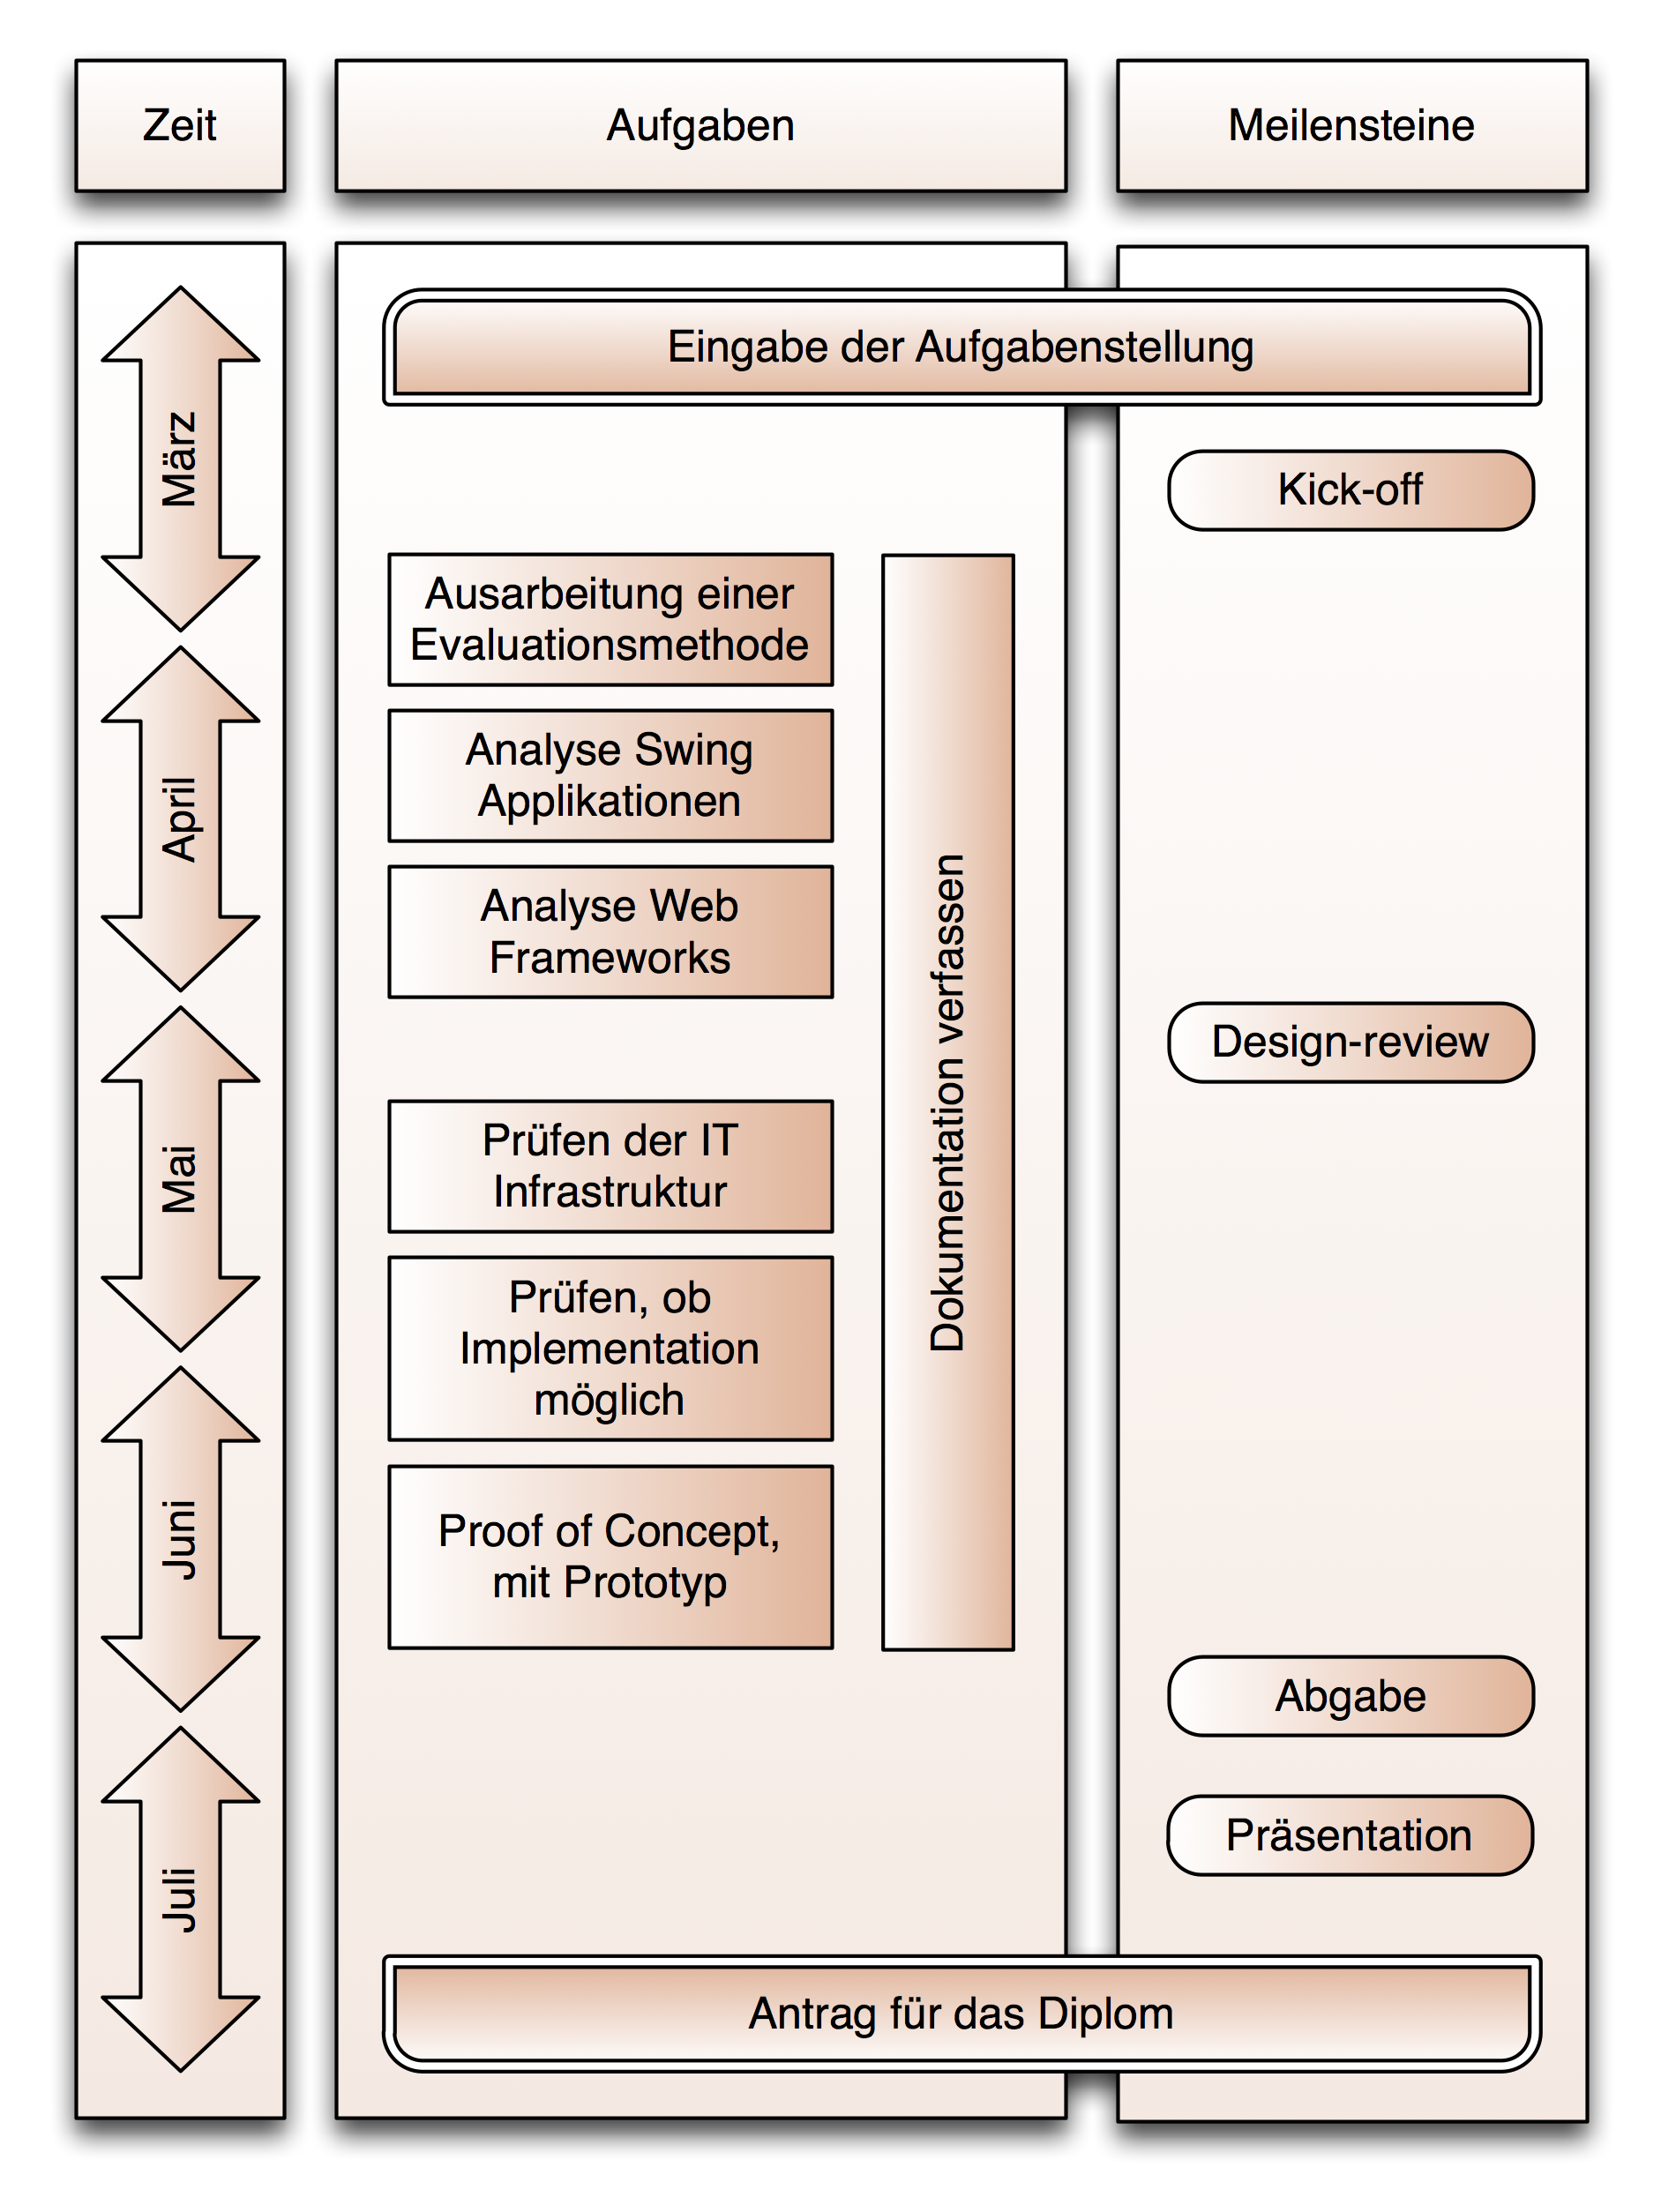
\includegraphics[width=0.7\textwidth]{./image/grobplanung.png}
      \caption{Chronologischer Ablauf der Diplomarbeit}
      \label{img:grobplanung}
    \end{center}
  \end{figure}
  
  \subsection{Aufwandschätzung}
  
  Die Aufwandschätzung soll mit realistischen Zeiten auf halbe Stunden
  genau gemacht werden. Zudem soll die effektiv gebraucht Zeit im Laufe der
  Diplomarbeit ergäntzt werden. Der gesamte Aufwand wird in fünf Gruppen
  unterteilt und ist in der Tabelle \ref{tab:planing} ersichtlich.
  \newline
  
  \begin{table}[ht]
    \begin{center}
      \begin{tabular}{p{9cm}rr}
        \toprule
        Arbeitspaket & Geplant & Effektiv \\
        \midrule
        Präsentationen &
        20.0 h &
        \ldots\\
        Gestellte Aufgaben gemäss Aufgabenstellung &
        147.0 h &
        \ldots\\
        Abzugebende Dokumente &
        94.0 h &
        \ldots\\
        Fachbetreuung durch den Dozenten &
        10.0 h &
        \ldots\\
        Administrative Aufgaben &
        13.5 h &
        \ldots\\
        \bottomrule
        Total &
        284.5 h &
        \ldots\\
        \bottomrule
      \end{tabular}
      \caption{Aufwandschätzung der Diplomarbeit}
      \label{tab:planing}
    \end{center}
  \end{table}
  
  \subsubsection{Präsentationen}
  
  Gemäss \cite{KillerPresentation} Slide 37f. braucht man für eine Stunde
  Präsentationszeit mindestens eine Vorbereitungszeit von 30 Stunden. Somit kann
  man das linear herunter brechen auf eine Stunde Vorbereitungszeit pro zwei
  Minuten Präsentationszeit. Die Planung ist in der Tabelle
  \ref{tab:presentationPlaning} ersichtlich.
  \newline
  
  \begin{table}[ht]
    \begin{center}
      \begin{tabular}{p{9cm}rr}
        \toprule
        Arbeitspaket & Geplant & Effektiv \\
        \midrule
        Kick-off Präsentation ca. 5 Minuten &
        2.5 h &
        4.0 h\\
        Design-review Präsentation ca. 10 Minuten &
        5.0 h &
        \ldots\\
        Schlusspräsentation ca. 20 Minuten &
        10.0 h &
        \ldots\\
        Prototyp Demo ca. 5 Minuten &
        2.5 h &
        \ldots\\
        \bottomrule
        Total &
        20.0 h &
        \ldots\\
        \bottomrule
      \end{tabular}
      \caption{Geplante Zeit für Präsentationen}
      \label{tab:presentationPlaning}
    \end{center}
  \end{table}
  
  \newpage
  
  \subsubsection{Gestellte Aufgaben gemäss Aufgabenstellung}
  
  Die einzelnen Aufgaben sollen in deren Teilaufgaben unterteilt werden. Die
  Planung ist in der Tabelle \ref{tab:aufgabenPlaning} ersichtlich.
  \newline
  
  \begin{table}[!h]
    \begin{center}
      \begin{tabular}{lp{7cm}rr}
        \toprule
        Aufgabe & Arbeitspaket & Geplant & Effektiv \\

        \midrule
        \ref{itm:Aufgabe-01} &
        Research zu Analyseverfahren von Java Swing Applikationen &
        8.0 h &
        \ldots\\
        &
        Definition des Analyseverfahrens &
        4.0 h &
        \ldots\\
        &
        Analyse von drei Java Swing Applikationen, à 4 Stunden &
        12.0 h &
        \ldots\\

        \midrule
        \ref{itm:Aufgabe-02} &
        Research zu Java Swing Komponenten &
        4.0 h &
        \ldots\\
        &
        Analyse von drei Java Swing Applikationen, à 2 Stunden &
        6.0 h &
        \ldots\\

        \midrule
        \ref{itm:Aufgabe-03} &
        Research zu Evaluationsverfahren im Bereich von Java Web Frameworks &
        12.0 h &
        \ldots\\
        &
        Definition des Evaluationsverfahrens &
        8.0 h &
        \ldots\\
        &
        Evaluation von fünf Java Web Frameworks, à 4 Stunden &
        20.0 h &
        \ldots\\

        \midrule
        \ref{itm:Aufgabe-04} &
        Analyse der IT Architektur der ZKB &
        8.0 h &
        \ldots\\
        &
        Prüfen ob die Integration möglich ist bei fünf Java Web Frameworks, à 2
        Stunden &
        10.0 h &
        \ldots\\
        
        \midrule
        \ref{itm:Aufgabe-05} &
        Analyse der Komponenten von fünf Java Web Frameworks und prüfen ob die
        Implementation möglich ist, à 3 Stunden &
        15.0 h &
        \ldots\\
        
        \midrule
        \ref{itm:Aufgabe-06} &
        Anforderungen an den Prototyp definieren &
        8.0 h &
        \ldots\\
        &
        Testfälle für den Prototyp definieren &
        8.0 h &
        \ldots\\
        &
        Umsetzung des Prototypen &
        20.0 h &
        \ldots\\
        &
        Empfehlung eines Java Web Frameworks &
        4.0 h &
        \ldots\\
        \bottomrule
        &
        Total &
        147.0 h &
        \ldots\\
        \bottomrule
      \end{tabular}
      \caption{Geplante Zeit für gestellte Aufgaben}
      \label{tab:aufgabenPlaning}
    \end{center}
  \end{table}
  
  \newpage
  
  \subsubsection{Abzugebende Dokumente}
  
  Gemäss den Bestimmungen für die Diplomarbeit, siehe \cite{hsz_reglement} S. 3,
  müssen einige Dokumente erstellt und abgegeben werden. Die Planung ist in der
  Tabelle \ref{tab:documentationPlaning} ersichtlich.
  \newline
  
  \begin{table}[ht]
    \begin{center}
      \begin{tabular}{p{9cm}rr}
        \toprule
        Arbeitspaket & Geplant & Effektiv \\
        \midrule
        Bericht in \LaTeX{} aufsetzen &
        10.0 h &
        \ldots\\
        Bericht in \LaTeX{} verfassen &
        60.0 h &
        \ldots\\
        Poster für die Diplomausstellung im A0 Format &
        16.0 h &
        \ldots\\
        Zusammenfassung à zwei A4-Seiten &
        8.0 h &
        \ldots\\
        \bottomrule
        Total &
        94.0 h &
        \ldots\\
        \bottomrule
      \end{tabular}
      \caption{Geplante Zeit für Dokumentation}
      \label{tab:documentationPlaning}
    \end{center}
  \end{table}
  
  \subsubsection{Fachbetreuung durch den Dozenten}
  
  Gemäss den Bestimmungen für die Diplomarbeit, siehe \cite{hsz_reglement} S. 2,
  stehen dem Diplomand zehn Stunden Betreuungszeit durch den Dozenten zur
  Verfügung. Die Planung ist in der Tabelle \ref{tab:observationPlaning}
  ersichtlich.
  \newline
  
  \begin{table}[ht]
    \begin{center}
      \begin{tabular}{p{9cm}rr}
        \toprule
        Arbeitspaket & Geplant & Effektiv \\
        \midrule
        Kick-off Meeting &
        1.0 h &
        1.0 h\\
        Design-review Meeting &
        1.0 h &
        \ldots\\
        Schlusspräsentation &
        1.0 h &
        \ldots\\
        Ausserterminliche Betreeuungszeit &
        7.0 h &
        \ldots\\
        \bottomrule
        Total &
        10.0 h &
        \ldots\\
        \bottomrule
      \end{tabular}
      \caption{Geplante Zeit für Betreuung}
      \label{tab:observationPlaning}
    \end{center}
  \end{table}
  
  \newpage
  
  \subsubsection{Administrative Aufgaben}
  
  Unter administrative Aufgaben fallen Tätigkeiten wie die Planung von Terminen,
  das Druckenlassen der Dokumentation, die Kommunikation mit der Schulleitung
  und dem Dozenten, usw. Auf Grund meiner Erfahrung mit Projekten, macht das in
  etwa fünf Prozent des gesamten Aufwandes aus.
  \newline
  
  \begin{table}[ht]
    \begin{center}
      \begin{tabular}{p{9cm}rr}
        \toprule
        Arbeitspaket & Geplant & Effektiv \\
        \midrule
        Planung von Terminen &
        2.0 h &
        \ldots\\
        Druckenlassen der Dokumentation &
        4.0 h &
        \ldots\\
        Kommunikation mit der Schulleitung und dem Dozenten &
        2.5 h &
        \ldots\\
        Übrige administrative Aufgaben &
        5.0 h &
        \ldots\\
        \bottomrule
        Total &
        13.5 h &
        \ldots\\
        \bottomrule
      \end{tabular}
      \caption{Geplante Zeit für administrative Aufgaben}
      \label{tab:administrationPlaning}
    \end{center}
  \end{table}
  
  \section{Arbeitsschritte}
  
  Alle vorgenommenen Arbeitsschritte werden in einem Wiki für die
  Nachvollziehbarkeit protokolliert. Das Wiki ist im Internet öffentlich
  zugänglich unter der \ac{URL}:
  \newline
  
  \url{https://github.com/sushicutta/Diplomarbeit/wiki/Arbeitsprotokoll}
  \newline
  
  \noindent
  Zusätzliche Informationen zum Ablauf der Diplomarbeit werden ebenfalls im Wiki
  erfasst und sind unter der \ac{URL} ersichtlich:
  \newline
  
  \url{https://github.com/sushicutta/Diplomarbeit/wiki/}
  
  \newpage
  
  \section{Meilensteine}
  
  Die Meilensteine entsprechen dem vorgegebenen Ablauf einer Diplomarbeit aus
  dem \ac{EBS}\footnote{\url{https://ebs.hsz-t.ch/}}. Die Projekt Termine wurden
  alle gemäss Reglement eingehalten, siehe Tabelle \ref{tab:milestones}.
  \newline
  
  \begin{table}[ht]
    \begin{center}
      \begin{tabular}{lp{7cm}ll}
        \toprule
        Datum & Meilenstein & Ort \\
        \midrule
        14. März 2011 &
        Die Aufgabenstellung zur Diplomarbeit wurde eingereicht &
        \ac{EBS}\\
        15. März 2011 &
        Freigabe der Diplomarbeit &
        \ac{EBS}\\
        21. März 2011 &
        Inhaltliches Kick-off Meeting &
        Panter llc\\
        13. April 2011 &
        Offizielles Kick-off Meeting &
        HSZ-T\\
        04. Mai 2011 &
        Design-Review Meeting &
        HSZ-T\\
        xx. xx. 2011 &
        Abgabe der Dokumentation &
        HSZ-T\\
        xx. xx. 2011 &
        Schlusspräsentation &
        HSZ-T\\
        \bottomrule
      \end{tabular}
      \caption{Projekt Meilensteine}
      \label{tab:milestones}
    \end{center}
  \end{table}
  
  \newpage
  
  \section{Erreichte Ziele}
  
  Es wurden alle Ziele gemäss den erwarteten Resultaten der Aufgabenstellung
  erreicht. Die einzelnen Punkte sind hier analog der Aufgabenstellung
  aufgeführt, siehe Tabelle \ref{tab:erreichteZiele}.
  \newline
  
  \begin{table}[ht]
    \begin{center}
      \begin{tabular}{lp{9cm}ll}
        \toprule
        Resultat & Ziel & Stand \\
        \midrule
        \ref{itm:Resultat-01} &
          Es soll eine Liste der erkannten GUI Paradigmen vorliegen. &
          offen\\
        \ref{itm:Resultat-02} &
          Es soll eine Liste der verwendeten Swingkomponenten vorliegen. &
          offen\\
        \ref{itm:Resultat-03} &
          Es soll eine Rangliste der fünf Frameworks, in der Anordnung
          entsprechend ihrer Eignung, vorliegen. &
          offen\\
        \ref{itm:Resultat-04} &
          Es sollen die Java Web Frameworks aufgelistet werden, welche für
          einen Einsatz in der IT Infrastruktur der Zürcher Kantonalbank in
          Frage kommen. &
          offen\\
        \ref{itm:Resultat-05} &
          Es sollen die Java Web Frameworks aufgelistet werden, welche die
          notwendigen Swingkomponenten und GUI Paradigmen unterstützen. &
          offen\\
        \ref{itm:Resultat-06} &
          Ein lauffähiger Prototyp. &
          offen\\
        \ref{itm:Resultat-07} &
          Es soll eine Empfehlung eines Java Web Frameworks, für den möglichen
          Einsatz in der Zürcher Kantonalbank, ausgesprochen werden. &
          offen\\
        \bottomrule
      \end{tabular}
      \caption{Übersicht der erreichten Ziele}
      \label{tab:erreichteZiele}
    \end{center}
  \end{table}